\documentstyle[11pt,fullpage,psfig]{article}
\begin{document}
\bibliographystyle{unsrt}

\title{Maximum likelihood fitting of extreme value distributions}
\author{Sean R. Eddy\\
Dept. of Genetics, Washington University School of Medicine\\
eddy@genetics.wustl.edu}
\date{14 November 1997}
\maketitle

\begin{abstract}
I discuss maximum likelihood fitting of extreme value distributions,
with an emphasis on applications in evaluating the statistical
significance of sequence or structural alignment scores. The aim is
not to present any novel theory. The techniques in this report are
well known in the literature, accessible to competent mathematicians,
and have already been applied in some computational biology
applications. Rather, my aim is to review the maximum likelihood
method in a form that is easily implemented in computational sequence
analysis software. As a source for specific examples, I use the
implementation of E-value calculations in the profile hidden Markov
model software package HMMER.
\end{abstract}

\section{Introduction}

In database search applications in computational biology, we generally
wish to determine the statistical significance of a score. This score
may be determined by a variety of methods. It may be a sequence
alignment score or a structural threading score; it may be the result
of an ad hoc scoring system or it may be the log probability under a
probabilistic model such as a hidden Markov model. Regardless of the
means used to arrive at the score, we will wish to know what the
probability is that we would see a given score by chance in a database
of negative (nonhomologous) sequences.

These statistical measures are represented as ``P-values'' or
``E-values''. A P-value is the {\em probability} of seeing at least
one score $S$ greater than or equal to some score $x$ in a database
search of $n$ sequences; we will use the symbol ${\cal P}(x,n)$ to
mean a P-value.  An E-value is the {\em expected number} of
nonhomologous sequences with scores greater than or equal to a score
$x$ in a database of $n$ sequences; we will use the symbol ${\cal
E}(x,n)$ to mean an E-value. The two measures are trivially obtained
from the probability $P(S \geq x)$ that any {\em single} nonhomologous
sequence scores better than or equal to $x$:

\begin{eqnarray*}
	{\cal P}(x,n) & = & 1 - e^{-nP(S \geq x)} \\
	{\cal E}(x,n) & = & nP(S \geq x)
\end{eqnarray*}

We therefore need a solution for $P(S \geq x)$, the distribution of
the score statistic $x$.

In computational biology, analytical solutions for the distribution
$P(S \geq x)$ only exist for ungapped local alignments, where the
distribution is an {\em extreme value distribution} (EVD).  In the
case of gapped local alignments, simulations indicate that these
scores also roughly obey an extreme value distribution, but the
relevant parameters can only be determined by simulation and empirical
curve-fitting. Programs such as {\sc FASTA}, the new gapped alignment
versions of {\sc BLAST}, several implementations of the Smith/Waterman
algorithm, and some other search algorithms use such techniques to fit
observed score distributions to an EVD.

Perhaps the simplest fitting method to implement is the {\em linear
regression} method. However, as shown below, the linear regression
method is markedly inferior to a second approach, {\em maximum
likelihood}. Maximum likelihood fitting to the extreme value
distribution has been described in the literature by Mott
\cite{Mott92} and in a textbook by Lawless \cite{Lawless82} (and
undoubtedly other places), and is now the technique used by the NCBI
gapped {\sc BLAST} software. 

The purpose of this paper is to write up my notes on the
implementation of maximum likelihood fitting of the extreme value
distribution in HMMER. The format is deliberately an ``EVD for poets''
presentation. The goal is to obviate the need for any differential
calculus on the part of a software implementor, and to simply give an
almost pseudocode implementation of the necessary methods.

\section{The extreme value distribution}

The probability density function (pdf) and the distribution function
of the extreme value distribution are:

\begin{equation}
P(x) = \lambda \exp \left[ -\lambda (x - \mu) - e^{- \lambda (x - \mu)} \right]
\label{eqn:density}
\end{equation}

\begin{equation}
P(S < x) = \exp \left[ -e^{-\lambda(x - \mu)} \right]
\label{eqn:distribution}
\end{equation}

The particular form of these equations follows Altschul and Gish
\cite{AltschulGish96}. The theory developed in these notes is taken
from a book by Lawless \cite{Lawless82}, a source recommended by
Altschul (personal communication). In Lawless, the EVD is described by
parameters $u$ and $b$, and is ``backwards'' (longer tail to the
left); use $(x - u) = -(x - \mu)$ and $b = 1 / \lambda$ to convert
Lawless' notation to that of Altschul and Gish. The extreme value
density and distribution functions for $\mu = 0$ and $\lambda = 1.0$
are shown below.

\centerline{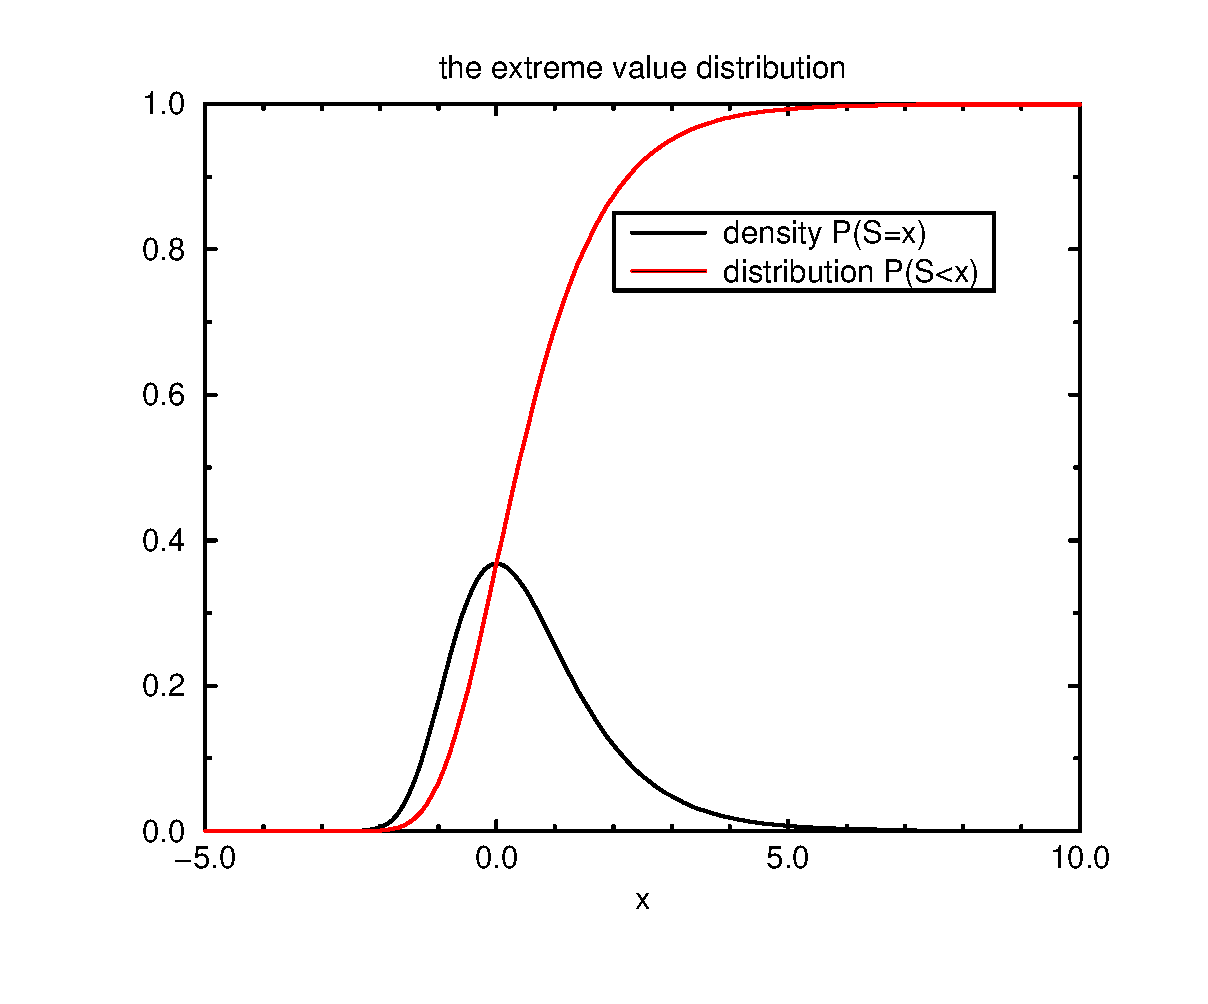
\psfig{file=evd_basic.eps,width=3in}}

\pagebreak
The $\mu$ and $\lambda$ parameters are {\em location} and {\em scale}
parameters, respectively. Their effects are shown in following figures.

\centerline{
\begin{minipage}{3in}
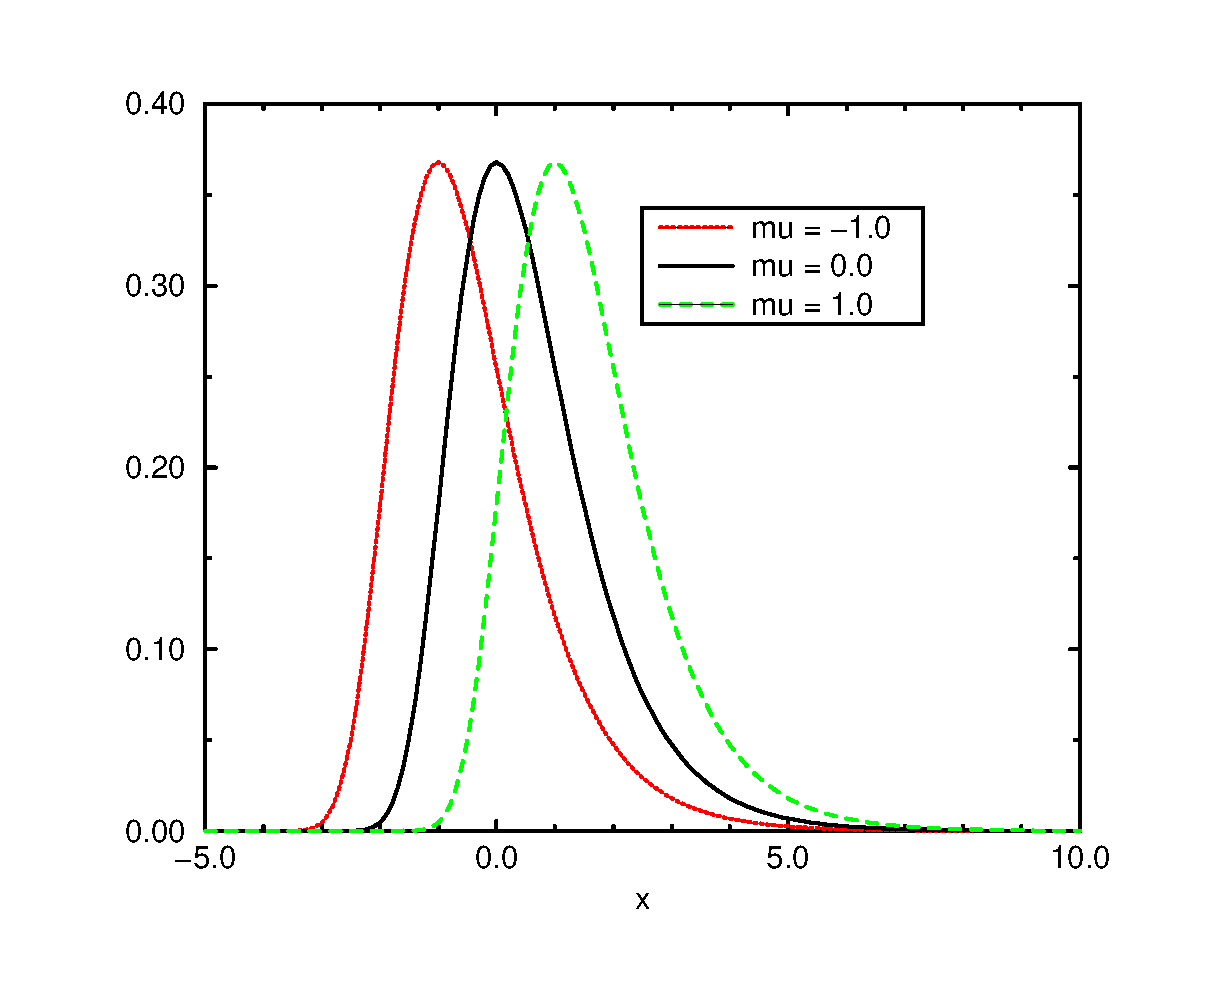
\psfig{file=evd_location.eps,width=2.8in}
\end{minipage}
\begin{minipage}{3in}
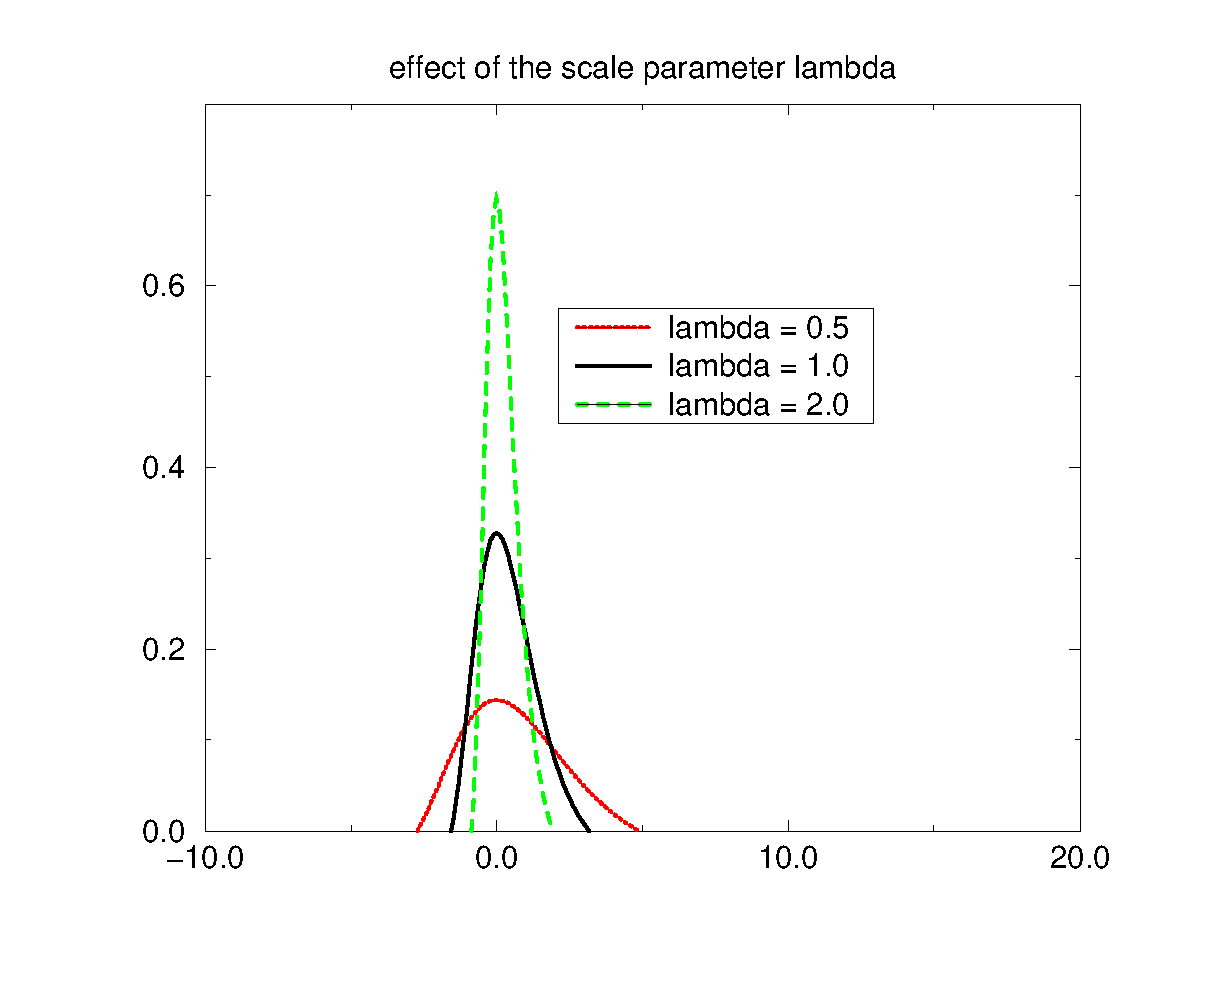
\psfig{file=evd_scale.eps,width=2.8in}
\end{minipage}
}

These plots were generated by a simple C program {\tt evd.c}, where
the key lines are:
\begin{verbatim}
                                /* density function P(S=x) */
      px = lambda * exp(-1.*lambda * (x - mu) - exp(-1* lambda * (x - mu)));
                                /* distribution function P(S < x) */
      psx= exp(-1* exp(-1*lambda * (x - mu)));
\end{verbatim}

\section{Fitting the EVD, 1: Linear regression}

A fast, simple method of fitting observed data to the EVD is by linear
regression fit to a $\log \log$ transformation of the $P(S < x)$
histogram:

\begin{equation}
\log \left[ -\log P(S<x) \right] = -\lambda x + \lambda \mu
\end{equation}

This is a straight line with slope $-\lambda$, $y$ intercept $\lambda
\mu$, and $x$ intercept $\mu$. Any canned linear regression routine
can quickly fit this line; e.g. {\tt fit()} in {\em Numerical Recipes
in C} \cite{Press88} or {\tt Linefit()} in the {\tt SQUID} library.

The trouble with linear regression is that it is not robust. Outliers
have a strong influence.  An example is shown below, in which I
generated $N$ EVD samples with $\mu = -20$, $\lambda = 0.4$ ({\tt
EVDrandom()}) , collated a histogram (using the {\tt histogram.c}
functions), fitted it by linear regression (\verb+EVDBasicFit()+), and
calculated \% deviation of the estimated $\mu$ and $\lambda$ from the
original parametric $\mu$ and $\lambda$. This experiment was repeated
500 times for four values of $N$, and the average and maximum
deviations were kept for each $N$.%
\footnote{See the testdriver {\tt Shiva/evd\_test.c}, RCS 1.1,
which uses EVD code in {\tt histogram.c}, RCS 1.3.
An example command line: 
\verb+ testdriver -v -n 500 -m 10000 | grep "error on lambda" | avg.perl+}
The results of this experiment were:

\begin{center}
\begin{tabular}{lrrrr} \hline
 & \multicolumn{4}{c}{\# samples in EVD histogram}\\
                        & 100 & 1000  & 10,000 & 100,000 \\
\% error in $\mu$       &  2\%&   1\% & 0.9\%  &  0.9\%  \\
max error in $\mu$      & 24\%&  13\% &  10\%  &   10\%  \\
\% error in $\lambda$   & 12\%&   7\% &   5\%  &    3\%  \\
max error in $\lambda$  & 49\%&  33\% &  25\%  &   20\%  \\ \hline
\end{tabular}
\end{center}

Plots of the fits from one such simulation experiment are shown
below. The example was chosen to be somewhat worse than the average
case, to emphasize the source of the error. Outliers in the tail occur
with significant probability and confound the regression fit.

\centerline{
\begin{minipage}{3in}
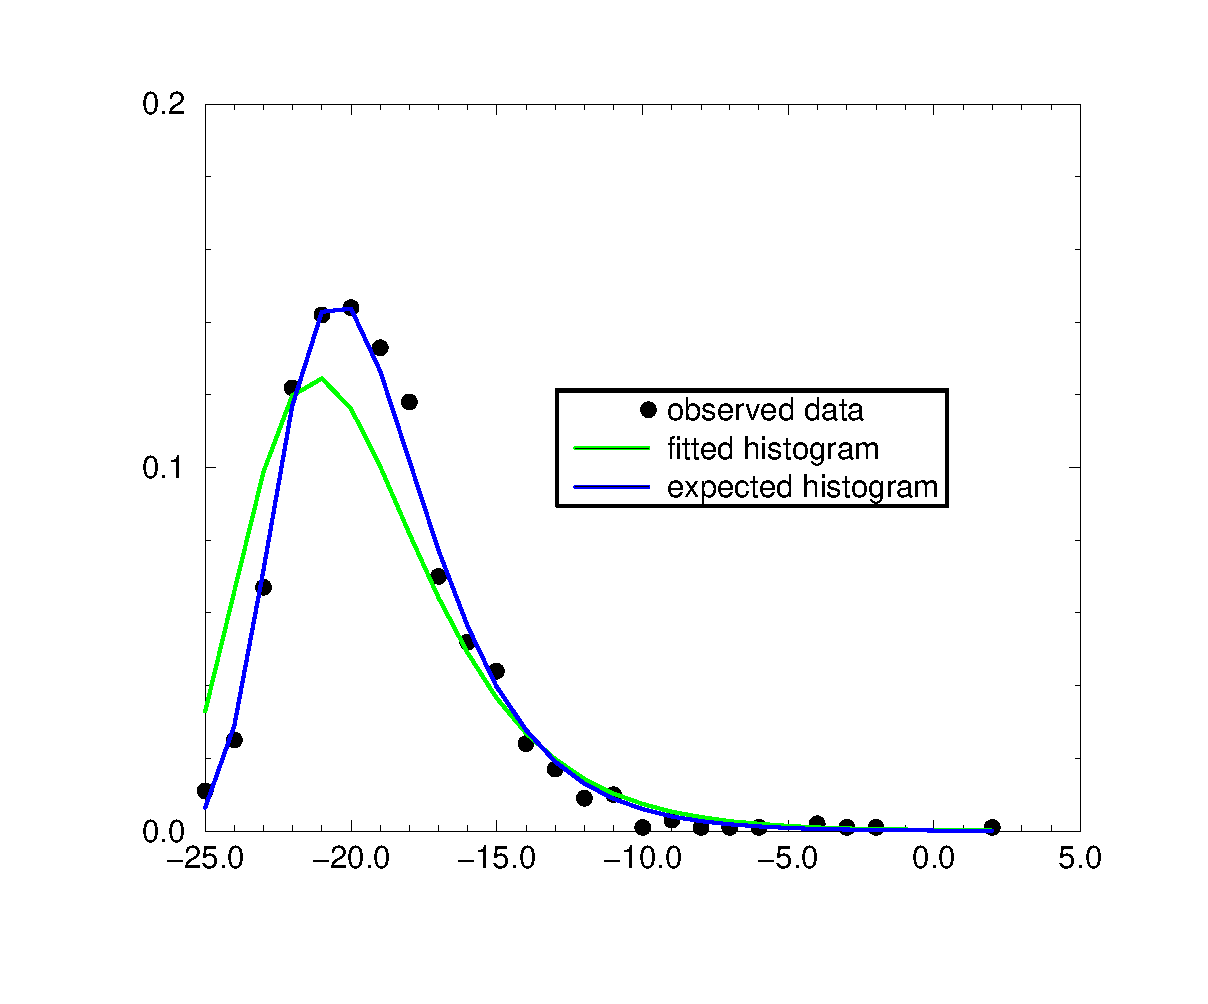
\psfig{file=evd_regression1.eps,width=2.8in}
\end{minipage}
\begin{minipage}{3in}
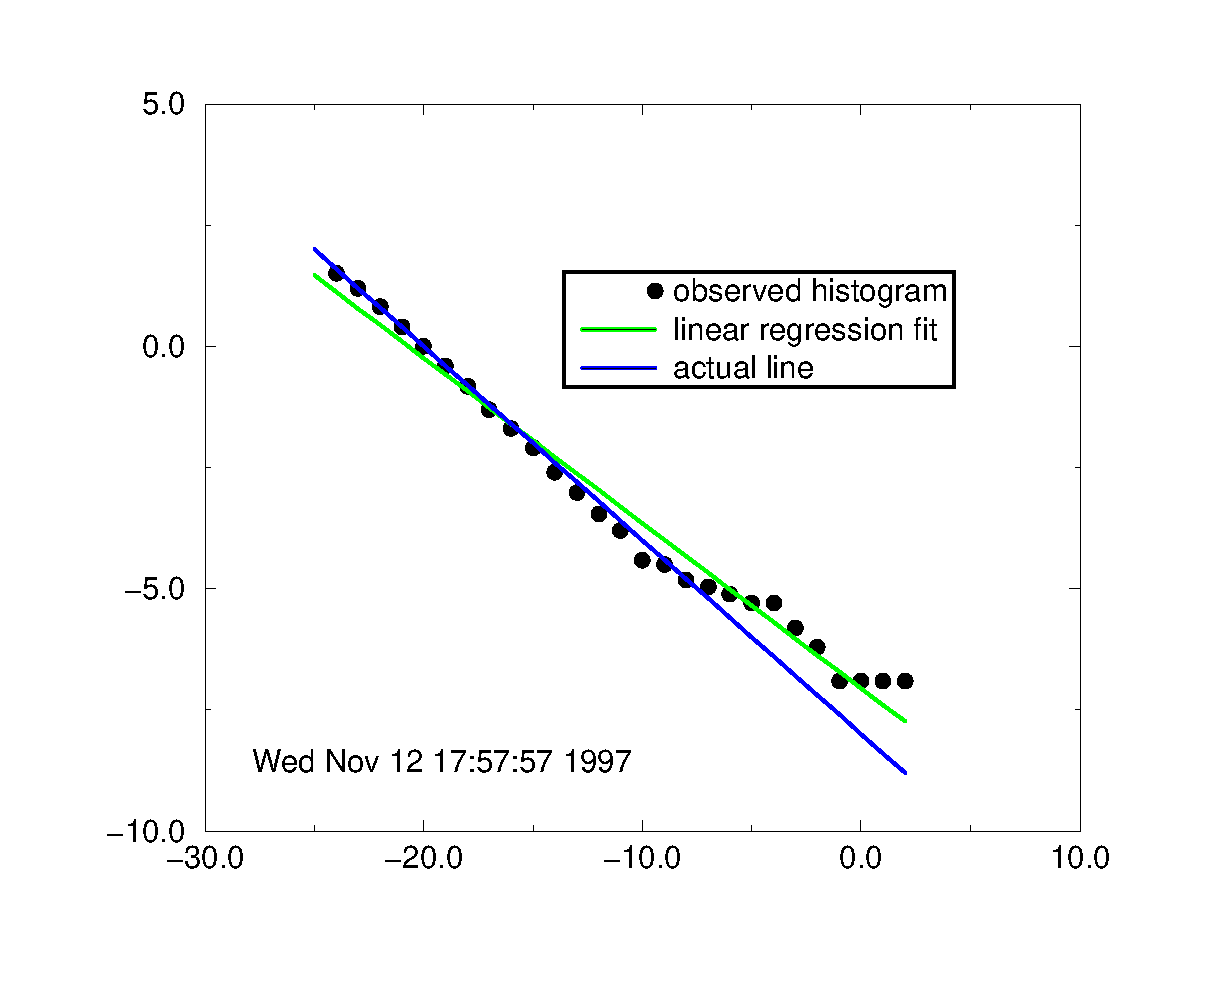
\psfig{file=evd_regression2.eps,width=2.8in}
\end{minipage}
}

We could imagine schemes to work around the non-robustness. For
example, a weighted linear regression ({\tt WeightedLinefit()}) might
be tried with high variances on poorly populated points.  It is also
possible to directly optimize a chi-squared fit to the histogram by a
brute force grid search (see {\tt histogram.c:evd\_bruteforce()}).
Early prototypes of HMMER2 used such schemes.

\section{Fitting the EVD, 2: Maximum likelihood}

The definitive guide to the theory of maximum likelihood fits to the
EVD appears to be Lawless \cite{Lawless82}. I first give the
derivation of the relevant equations in (extreme) detail. Lawless does
not (and besides, uses a different notation than Altschul and Gish)
and I had to convince myself of the correctness of the derivation;
second, I don't trust my algebra, so this is my permanent record if I
forget how it all worked; and third, some necessary details were
missing from Lawless and had to be derived. Only three of the
equations derived in this section are actually needed in an
implementation: (\ref{eqn:solvemu}), (\ref{eqn:newtontarget}), and
(\ref{eqn:newtonderivative}).  The algorithm in the implementation is
then summarized, and some results of simulations are given.

\subsection{Mathematical derivations}

The likelihood of drawing $n$ samples $x_i$ from an extreme value
distribution with parameters $\lambda$ and $\mu$ is:

\[
P(x_1 \ldots x_n | \lambda, \mu) = 
\prod_{i=1}^{n} \lambda \exp \left[ 
-\lambda(x_i - \mu) - e^{-\lambda(x_i - \mu)} \right]
\]

which is readily rearranged to give:

\begin{equation}
P(x_1 \ldots x_n | \lambda, \mu) =
\lambda^n \exp \left[ \sum_{i=1}^{n} -\lambda(x_i - \mu) 
	- \sum_{i=1}^{n} e^{-\lambda(x_i - \mu)} \right]
\end{equation}

The log likelihood $\log L(\lambda, \mu) = \log P(x_1 \ldots x_n | \lambda, \mu)$ is:
\begin{equation}
\log L(\lambda, \mu) = 
n \log \lambda - \sum_{i=1}^{n} \lambda(x_i - \mu) 
- \sum_{i=1}^{n} e^{-\lambda(x_i - \mu)}
\label{eqn:logL}
\end{equation}

In a maximum likelihood fitting approach, our goal is to find
$\hat{\lambda}$ and $\hat{\mu}$ that maximize the log likelihood $\log
L(\lambda, \mu)$. A brute force fit is possible, since there are only two
parameters, but it is more efficient to get partial first derivatives
from $\log L(\lambda,\mu)$ so a more directed optimization can be done:

\begin{eqnarray}
\frac{\partial \log L}{\partial \mu} & = &
n \lambda - \lambda \sum_{i=1}^{n} e^{-\lambda (x_i - \mu)}
\label{eqn:mupartial}
\\%
\frac{\partial \log L}{\partial \lambda} & = &
\frac{n}{\lambda} - \sum_{i=1}^{n} (x_i - \mu) +  
\sum_{i=1}^{n} (x_i - \mu) e^{-\lambda (x_i - \mu)}
\label{eqn:lambdapartial}
\end{eqnarray}

The maximum likelihood estimates $\hat{\lambda}$ and $\hat{\mu}$ are
the solutions to $\frac{\partial \log L}{\partial \mu} = 0$ and
$\frac{\partial \log L}{\partial \lambda} = 0$. Lawless gives a useful
trick here, in which we only need to solve one equation instead of
two.  Observe that when (\ref{eqn:mupartial}) is set to zero, it can be
used to get $\hat{\mu}$ in terms of $\hat{\lambda}$:

\begin{eqnarray}
n \hat{\lambda} - \hat{\lambda} \sum_{i=1}^{n} e^{-\hat{\lambda} (x_i - \hat{\mu})} & = & 0 \nonumber \\
%
\sum_{i=1}^{n} e^{-\hat{\lambda} (x_i - \hat{\mu})} & = & n \nonumber\\
%
\sum_{i=1}^{n} e^{-\hat{\lambda} x_i} e^{\hat{\lambda} \hat{\mu}} & = & n \nonumber\\
%
e^{\hat{\lambda} \hat{\mu}} \sum_{i=1}^{n} e^{-\hat{\lambda} x_i} & = & n \nonumber\\
%
e^{-\hat{\lambda} \hat{\mu}} & = & \frac{1}{n} \sum_{i=1}^{n} e^{-\hat{\lambda} x_i} 
\label{eqn:substitute}\\
%
e^{\hat{\mu}} & = & \left[ \frac{1}{n} \sum_{i=1}^{n}
e^{-\hat{\lambda} x_i} \right]^{-\frac{1}{\hat{\lambda}}}
\nonumber \\
%
\mu & = & - \frac{1}{\lambda} 
	\log \left[ \frac{1}{n} \sum_{i=1}^{n} e^{-\hat{\lambda} x_i} \right]
\label{eqn:solvemu}
\end{eqnarray}

Now we can substitute (\ref{eqn:substitute}) into
(\ref{eqn:lambdapartial}), and look for an equation that gives us
$\hat{\lambda}$ in terms of the $x_i$'s:

\begin{eqnarray}
\frac{n}{\hat{\lambda}} - \sum_{i=1}^{n} (x_i - \hat{\mu}) +  
\sum_{i=1}^{n} (x_i - \hat{\mu}) e^{-\hat{\lambda} (x_i - \hat{\mu})} 
& = & 0
\nonumber \\
%
\frac{n}{\hat{\lambda}} - \sum_{i=1}^{n} x_i + \sum_{i=1}^{n} \hat{\mu} +
\sum_{i=1}^{n} (x_i - \hat{\mu}) e^{-\hat{\lambda} x_i} e^{\hat{\lambda}\hat{\mu}} 
& = & 0
\nonumber \\
%
\frac{n}{\hat{\lambda}} - \sum_{i=1}^{n} x_i + n \hat{\mu} +
\frac{\sum_{i=1}^{n} (x_i - \hat{\mu}) e^{-\hat{\lambda} x_i}} 
     {e^{-\hat{\lambda}\hat{\mu}}}
& = & 0
\nonumber \\
%
\frac{n}{\hat{\lambda}} - \sum_{i=1}^{n} x_i + n \hat{\mu} +
\frac{\sum_{i=1}^{n} (x_i - \hat{\mu}) e^{-\hat{\lambda} x_i}} 
     {\frac{1}{n} \sum_{i=1}^{n} e^{-\hat{\lambda} x_i}}
& = & 0
\nonumber \\
%
\frac{n}{\hat{\lambda}} - \sum_{i=1}^{n} x_i + n \hat{\mu} +
\frac{n \sum_{i=1}^{n} x_i e^{-\hat{\lambda} x_i} - n \hat{\mu} \sum_{i=1}^{n}
e^{-\hat{\lambda} x_i}}
     {\sum_{i=1}^{n} e^{-\hat{\lambda} x_i}}
& = & 0
\nonumber \\
%
\frac{n}{\hat{\lambda}} - \sum_{i=1}^{n} x_i + n \hat{\mu} +
\frac{n \sum_{i=1}^{n} x_i e^{-\hat{\lambda} x_i}}
     {\sum_{i=1}^{n} e^{-\hat{\lambda} x_i}} 
- n\hat{\mu}
& = & 0
\nonumber \\
%
\frac{1}{\hat{\lambda}} - \frac{1}{n} \sum_{i=1}^{n} x_i +
\frac{\sum_{i=1}^{n} x_i e^{-\hat{\lambda} x_i}}
     {\sum_{i=1}^{n} e^{-\hat{\lambda} x_i}} 
& = & 0
\label{eqn:newtontarget}
\end{eqnarray}

This line is well-behaved in the vicinity of the root, as shown below
for a simulation of 1000 samples from an EVD with $\lambda = 0.4$ and
$\mu = -20$ ($\lambda$ is varied along the X axis):

\centerline{
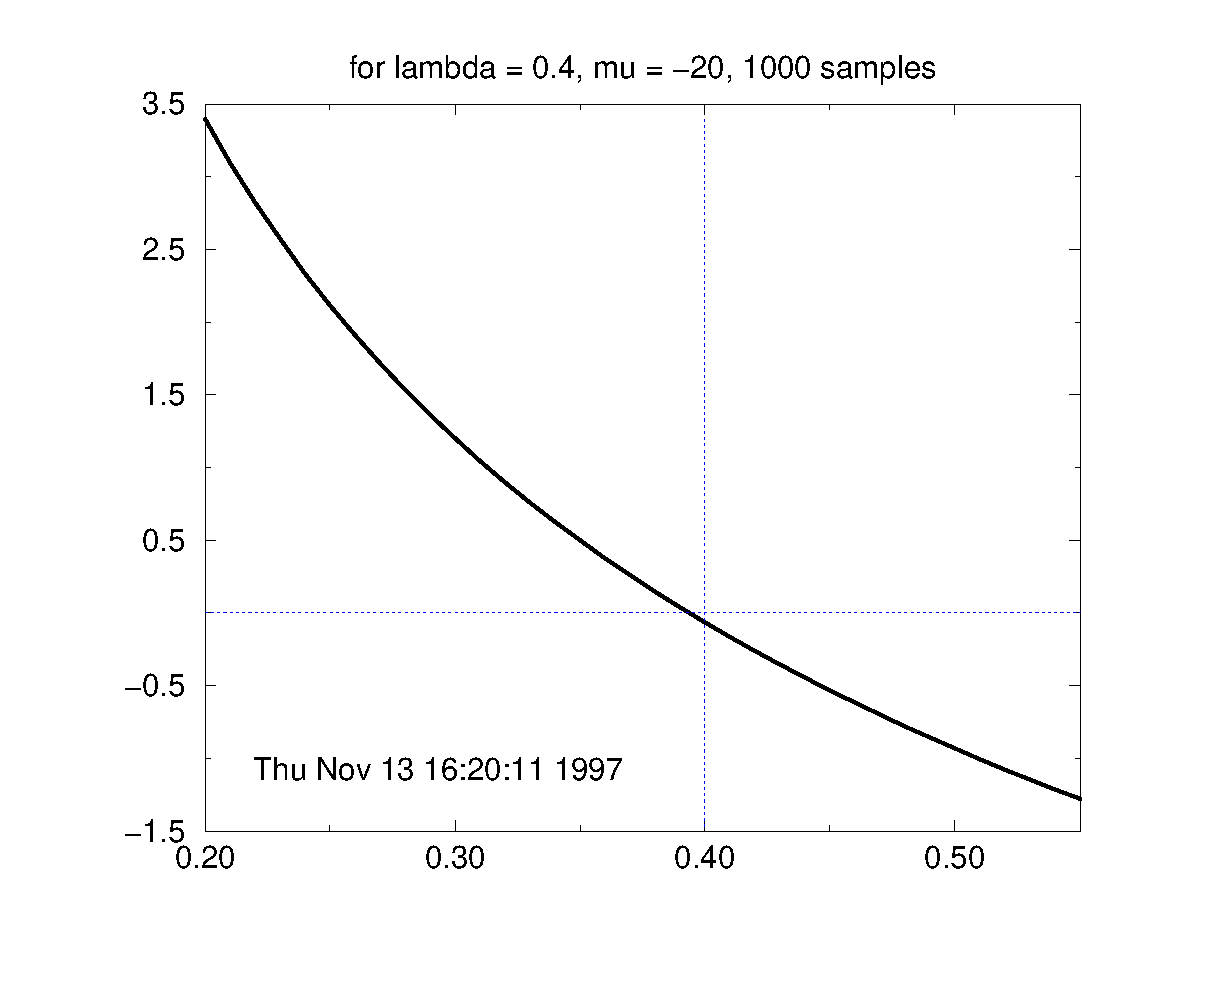
\psfig{file=evd_mlsolve.eps,width=3in}
}

\subsection{Solving for the root of (\ref{eqn:newtontarget})}

Because it is well-behaved, we can apply a fast Newton-Raphson
algorithm to find the root. We need the first derivative of
(\ref{eqn:newtontarget}) to use Newton-Raphson. It turns out that
Lawless does not give the derivative -- hence, one of the reasons I
had to put some effort into this, since I'm calculus-impaired -- but
it is relatively easy to derive. Recall from the algebra of
derivatives that:

\[
\left( \frac{f}{g} \right)' = \frac{g \cdot f' - f \cdot g'}{g^2}
\]

Starting from (\ref{eqn:newtontarget}), let:

\begin{eqnarray*}
f & = & \sum_{i=1}^{n} x_i e^{-\hat{\lambda} x_i}, \\
g & = & \sum_{i=1}^{n} e^{-\hat{\lambda} x_i}; \\
\end{eqnarray*}

and then differentiate $f$ and $g$ with respect to $\lambda$:

\begin{eqnarray*}
f' & = & - \sum_{i=1}^{n} x_i^2 e^{-\hat{\lambda} x_i}, \\
g' & = & - \sum_{i=1}^{n} x_i e^{-\hat{\lambda} x_i}. \\
\end{eqnarray*}

Differentiating (\ref{eqn:newtontarget}) is now straightforward,
and after minor rearrangement yields:

\begin{equation}
\frac{d}{d\lambda} = 
\frac{\left( \sum_{i=1}^{n} x_i e^{-\hat{\lambda} x_i} \right)^2 } 
     {\left( \sum_{i=1}^{n} e^{-\hat{\lambda} x_i}     \right)^2 }
-
\frac{\sum_{i=1}^{n} x_i^2 e^{-\hat{\lambda} x_i}}
     {\sum_{i=1}^{n} e^{-\hat{\lambda} x_i}}
-
\frac{1}{\hat{\lambda}^2}
\label{eqn:newtonderivative}
\end{equation}

\subsection{Implementation of ML EVD fitting}

For an implementation, the key equations are (\ref{eqn:solvemu}),
(\ref{eqn:newtontarget}), and (\ref{eqn:newtonderivative}). We also
need the Newton/Raphson algorithm (see \cite{Press88} for details) but
it turns out that a satisfactory implementation of Newton/Raphson only
takes a few lines of code. The algorithm is:

\begin{itemize}
\item Guess $\lambda$. (Linear regression fitting gives a very good
      guess, but the function appears to be so smooth that even
      random guesses, like $\lambda = 0.2$, seem to work fine.)
\item Apply Newton/Raphson to find the $\hat{\lambda}$ that satisfies
      (\ref{eqn:newtontarget}):
	\begin{itemize}
	\item calculate the target function $f$ and 
         its first derivative $f'$ at $\lambda$, using 
	(\ref{eqn:newtontarget}) to calculate $f$ and 
	(\ref{eqn:newtonderivative}) to calculate $f'$.
	\item If $f$ is within some absolute tolerance of zero 
	(e.g., $10^{-6}$), stop; we have found $\hat{\lambda}$.
	\item Else, estimate a new $\lambda = \lambda - \frac{f}{f'}$,
	  and do another iteration.
	\end{itemize}
\item Plug $\hat{\lambda}$ into (\ref{eqn:solvemu}) to get $\hat{\mu}$.
\end{itemize}

{\sc hmmer} implements basic algorithm in two functions.  {\tt
Lawless416()} calculates the target function and its first derivative,
given the current estimate of $\lambda$ (the name comes from Lawless'
equation 4.1.6, the target function). {\tt EVDMaxLikelyFit()} is a
no-frills implementation of the Newton/Raphson iterations and the
solution of $\hat{\mu}$.

\subsection{Results of ML EVD fits}

I repeated the experiment from the linear regression section, now
applying maximum likelihood fitting:

\begin{center}
\begin{tabular}{lrrrr} \hline
 & \multicolumn{4}{c}{\# samples in EVD histogram}\\
                        & 100 & 1000  & 10,000 & 100,000 \\
\% error in $\mu$       &  1\%& 0.3\% &  0.1\% & 0.03\%  \\
max error in $\mu$      &  4\%&   1\% &  0.4\% &  0.1\%  \\
\% error in $\lambda$   &  6\%&   2\% &  0.6\% &  0.2\%  \\
max error in $\lambda$  & 27\%&   7\% &  2.4\% &  0.9\%  \\ \hline
\end{tabular}
\end{center}

Maximum likelihood is significantly superior to linear regression for
fitting the EVD. The ML fit for 100 data points is better than the
linear regression fit for 10,000 data points.

\pagebreak
An example of a fairly ``bad'' ML fit (6\% error in $\hat{\lambda}$
for a 1000 point simulation) is shown below:

\centerline{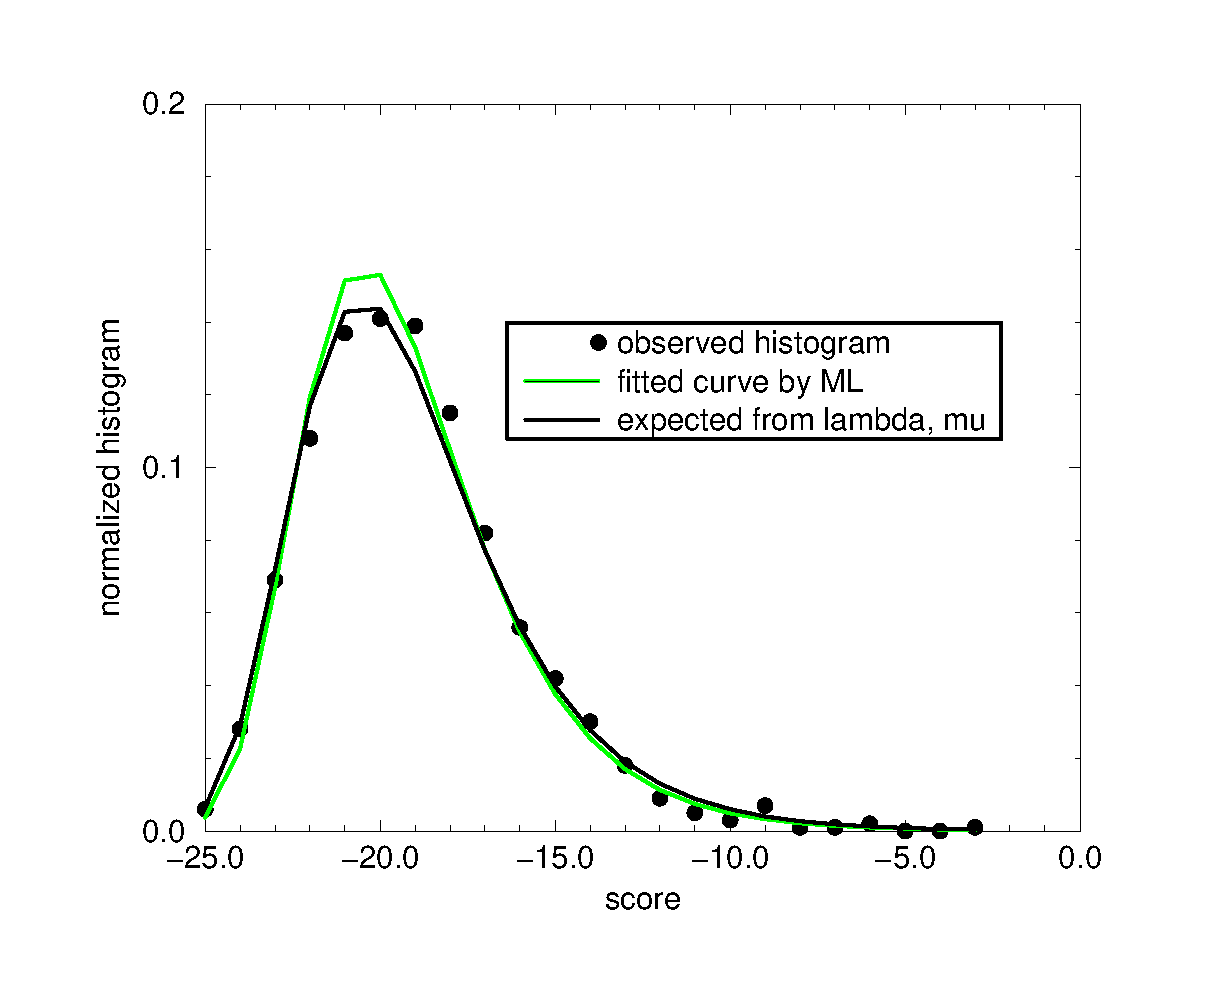
\psfig{file=evd_mlexample.eps,width=3in}}


%%%%%%%%%%%%%%%%%%%%%%%%%%%%%%%%%%%%%%%%%%%%%%%%%%%%%%%%%%%%
% Censored data. Lawless [1982], pp. 169-170
%%%%%%%%%%%%%%%%%%%%%%%%%%%%%%%%%%%%%%%%%%%%%%%%%%%%%%%%%%%%

\section{Fitting ``censored'' histograms to the EVD}

We may wish to fit only the right tail of the histogram, rather than
the whole histogram. For example, the left (low scoring) tail may be
contaminated with very poor-scoring sequences that do not conform to
the EVD, so we don't wish to include them in the fit. If, {\em a
priori}, we choose to cut off the data such that we do not include any
$x_i < c$ in the fit, we have a so-called ``Type I censored'' data set
\cite{Lawless82}.

In the equations that follow, let $c$ be the censoring value and $z$
be the number of censored samples, e.g. the number for which $x_{i} <
c$.

For the observed samples, their probability is still given by
(\ref{eqn:density}). For the censored samples, their probability is
given by (\ref{eqn:distribution}) -- the cumulative distribution at
$c$ gives us the probability of $x_i < c$. Therefore the probability of
a data set of $n$ observed samples and $z$ censored samples is:

\[
L(x_1 \ldots x_n, x_{n+1} \ldots x_{n+z} | \lambda, \mu) = 
\left( \prod_{i=1}^{n} \lambda \exp \left[ 
-\lambda(x_i - \mu) - e^{-\lambda(x_i - \mu)} \right]
\right)
\left(
\exp \left[ -e^{- \lambda (c - \mu)} \right]
\right)^z
\]

The log likelihood $L(\lambda, \mu)$ is then:

\begin{equation}
\log L(\lambda, \mu) = 
n \log \lambda 
- z e^{-\lambda(c - \mu)}
- \sum_{i=1}^{n} \lambda(x_i - \mu) 
- \sum_{i=1}^{n} e^{-\lambda(x_i - \mu)}
\label{eqn:censor_logL}
\end{equation}


Again, we wish to find $\hat{\lambda}$ and $\hat{\mu}$ that maximize
the likelihood. The form of (\ref{eqn:censor_logL}) is almost the same
as that of (\ref{eqn:logL}), so the procedure we follow is almost
identical. We need the first derivative of the likelihood with respect
to both parameters:

\begin{eqnarray}
\frac{\partial \log L}{\partial \mu} & = &
n \lambda  
- z \lambda e^{-\lambda (c - \mu)}
- \lambda \sum_{i=1}^{n} e^{-\lambda (x_i - \mu)}
\label{eqn:censor_dmu}
\\%
\frac{\partial \log L}{\partial \lambda} & = &
\frac{n}{\lambda} 
+ z (c - \mu) e^{-\lambda (c - \mu)}
- \sum_{i=1}^{n} (x_i - \mu) 
+ \sum_{i=1}^{n} (x_i - \mu) e^{-\lambda (x_i - \mu)}
\label{eqn:censor_dlambda}
\end{eqnarray}

Setting (\ref{eqn:censor_dmu}) to zero and solving for $\hat{\mu}$ in
terms of $\hat{\lambda}$ gives:

\begin{equation}
\mu  =  - \frac{1}{\lambda} 
	\log \left[ \frac{1}{n} 
	\left( z e^{-\hat{\lambda} c} 
               + \sum_{i=1}^{n} e^{-\hat{\lambda} x_i} \right)
	\right]
\label{eqn:censor_solvemu}
\end{equation}

Substituting (\ref{eqn:censor_solvemu}) into
(\ref{eqn:censor_dlambda}) gives us our target equation:

\begin{equation}
\frac{1}{\hat{\lambda}} 
- \frac{1}{n} \sum_{i=1}^{n} x_i +
\frac{z c e^{-\hat{\lambda} c} + \sum_{i=1}^{n} x_i e^{-\hat{\lambda} x_i}} 
     {z e^{-\hat{\lambda} c} + \sum_{i=1}^{n} e^{-\hat{\lambda} x_i}} 
 =  0
\label{eqn:censor_newtontarget}
\end{equation}

Finally, the first derivative of the target equation with respect to
$\lambda$ is:

\begin{equation}
\frac{d}{d\lambda} = 
\frac{\left( 
        z c e^{-\hat{\lambda} c}
        + \sum_{i=1}^{n} x_i e^{-\hat{\lambda} x_i} 
       \right)^2 } 
     {\left( 
        z e^{-\hat{\lambda} c}
        + \sum_{i=1}^{n} e^{-\hat{\lambda} x_i}     
       \right)^2 }
-
\frac{z c^2 e^{-\hat{\lambda} c} + \sum_{i=1}^{n} x_i^2 e^{-\hat{\lambda} x_i}}
     {z  e^{-\hat{\lambda} c} + \sum_{i=1}^{n} e^{-\hat{\lambda} x_i}}
-
\frac{1}{\hat{\lambda}^2}
\label{eqn:censor_newtonderiv}
\end{equation}

Given $n$ observed data points $x_{i = 1 \ldots n}$, the number $z$ of
censored samples, and the censoring cutoff $c$, we can now solve for
maximum likelihood estimates $\hat{\lambda}$ and $\hat{\mu}$ using the
same procedure we used for uncensored data, by substituting equations
(\ref{eqn:censor_solvemu}), (\ref{eqn:censor_newtontarget}), and
(\ref{eqn:censor_newtonderiv}) for equations (\ref{eqn:solvemu}),
(\ref{eqn:newtontarget}), and (\ref{eqn:newtonderivative}).

{\sc hmmer} implements equations (\ref{eqn:censor_newtontarget}) and
(\ref{eqn:censor_newtonderiv}) in {\tt Lawless422()}. The
Newton/Raphson iterations and equation (\ref{eqn:censor_solvemu}) are
implemented in {\tt EVDCensoredFit()}.

\section{Results}

The function {\tt ExtremeValueFitHistogram()} in {\sc hmmer} attempts
to do a robust EVD fit to an observed histogram. It censors the data
below the peak of the histogram, so it only fits the right side of the
curve (guarding against low-scoring outliers). Because it expects many
low-scoring outliers, it attempts to estimate $z$ rather than directly
counting $z$.  It removes outliers to the right first by cutting above
a given score ({\tt high\_hint}) and then iteratively lowers its cutoff
and reestimated $\mu$ and $\lambda$ until the high cutoff is at an
estimated E-value of 1. Finally, a certain loss of precision is
introduced because it fits to a binned histogram, rather than fitting
to a list of observed scores. 

On simulated EVD data with no noise, {\tt ExtremeValueFitHistogram()}
gives the following accuracies (EVD with $\mu = -20, \lambda = 0.4$,
500 simulations):

\begin{center}
\begin{tabular}{lrrrr} \hline
 & \multicolumn{4}{c}{\# samples in EVD histogram}\\
                        & 100 & 1000  & 10,000 & 100,000 \\
\% error in $\mu$       &  2\%& 0.6\% &  0.2\% &  0.1\%  \\
max error in $\mu$      & 15\%&   5\% &  0.6\% &  0.3\%  \\
\% error in $\lambda$   & 15\%&   3\% &  0.9\% &  0.3\%  \\
max error in $\lambda$  & 87\%&  16\% &    4\% &    1\%  \\ \hline
\end{tabular}
\end{center}

(One reason the accuracies degrade is that left-censoring removes
about 40\% of the data before the fitting occurs.)

10,000 samples seem to be sufficient for reasonable fits.

On simulated EVD data with noise injected on the high side, {\tt
ExtremeValueFitHistogram()} is moderately robust but can go squirrely
if a lot of noise is present: (1000 EVD samples with $\mu = -20,
\lambda = 0.4$; varying amount of Gaussian noise with mean 20,
std. dev. 20; 500 simulations)

\begin{center}
\begin{tabular}{lrrrrr} \hline
 & \multicolumn{4}{c}{\# samples of Gaussian noise}\\
                        & 0   &   10  &    50  &  100   & 500  \\
\% error in $\mu$       &0.6\%& 0.5\% &  0.8\% &    2\% &  4\% \\
max error in $\mu$      &  5\%&   5\% &    4\% &    4\% &  8\% \\
\% error in $\lambda$   &  3\%&   3\% &    4\% &    7\% & 68\% \\
max error in $\lambda$  & 21\%&  16\% &   17\% &   16\% & 74\% \\ \hline
\end{tabular}
\end{center}

However, compare that to the rapid degradation of straight ML
estimation (no censoring, no outlier removal):

\begin{center}
\begin{tabular}{lrrrrr} \hline
 & \multicolumn{4}{c}{\# samples of Gaussian noise}\\
                        & 0   &   10  &    50  &  100   & 500  \\
\% error in $\mu$       &0.3\%& 0.6\% &    3\% &    5\% &  27\% \\
max error in $\mu$      &  1\%&   2\% &    4\% &    7\% &  29\% \\
\% error in $\lambda$   &  2\%&   10\% &   36\% &   52\% &  81\% \\
max error in $\lambda$  &  8\%&  54\% &   72\% &   75\% &  83\% \\ \hline
\end{tabular}
\end{center}

\bibliography{master,new} 
\end{document}
